\chapter{Forwarder Receiver}
\section{Summary}
Das Forwarder-Receiver Pattern ermöglicht transparente Interprozesskommunikation für Peer-to-Peer-Systeme. Forwarder und Receiver Komponenten entkoppeln die Peers von den unterliegenden Kommunikationsmechanismen.

\section{Context}
Peer-to-Peer Kommunikation.

\section{Problem}
Ein gängiger Weg um verteilte Applikationen zu erstellen, ist die Verwendung von low-level Mechanismen für die Interprozesskommunikation wie bspw. TCP/IP, Sockets oder Message Queues. Diese sind effizienter als high-level Mechanismen wie z.B. Remote Procedure Calls. Allerdings führen die low-level Mechanismen oft zu Abhängigkeiten auf das Betriebssystem und die verwendeten Netzwerkprotokolle.

Das Forwarder-Receiver Pattern um ist nützlich um folgende Forces auszubalancieren:
\begin{itemize}
	\item Das System soll die Austauschbarkeit der Kommunikationsmechanismen ermöglichen.
	\item Die Kooperation der Komponenten folgt einem Peer-to-Peer Modell, in welchem der Sender lediglich den Namen des Empfängers kennen muss.
	\item Die Kommunikation zwischen den Peers soll keinen grossen Einfluss auf die Performance haben.
\end{itemize}

\section{Solution}
Verteilte Peers arbeiten zusammen an der Lösung eines bestimmten Problems. Ein Peer kann einerseits ein Client sein und Services anfordern oder ein Server sein und Services anbieten oder beides. Die Details der unterliegenden Kommunikationsmechanismen werden dabei vor den Peers versteckt indem sie separate Komponenten gekapselt werden.

\section{Structure}
Das Forwarder-Receiver Pattern besteht aus folgenden drei Komponenten:
\paragraph{Peer:} Peer Komponenten führen die eigentliche Aufgabe der Applikation aus. Dazu kommunizieren sie mit anderen Peers. Ein Peer kennt lediglich die Namen der anderen Peers mit denen es kommuniziert. Es verwendet einen Forwarder um Nachrichten zu verschicken und einen Receiver um Nachrichten zu empfangen.

\paragraph{Forwarder:} Die Forwarder Komponente bietet ein generelles Interface welches eine Abstraktion eines bestimmten Interprozesskommunikationsmechanismus ist und ist zuständig für das Umwandeln und Versenden von Nachrichten. Die Komponente verfügt über ein Name-to-Address-Mapping und kann somit den Peers anhand ihres Namens eine physische Adresse zuordnen.

\paragraph{Receiver:} Receiver Komponenten sind zuständig für das Empfangen und Umwandeln von Nachrichten.

\medskip
Die folgende Grafik zeigt das Zusammenspiel der Komponenten:
\begin{figure}[H]
	\centering
	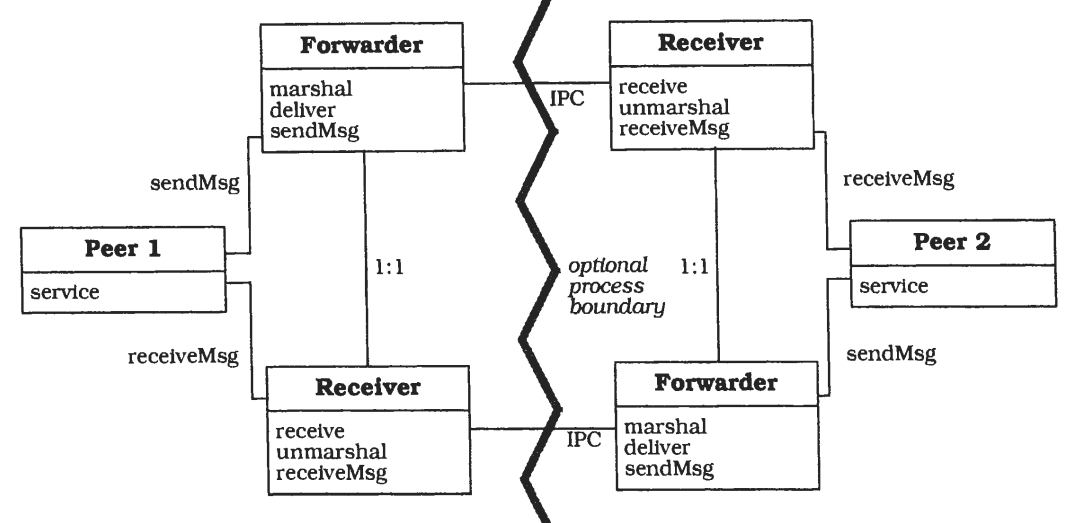
\includegraphics[width=0.8\textwidth]{figures/11-forwarder-receiver-1.png}
	\caption{View Handler Komponenten}
\end{figure}


\section{Variants}
\begin{itemize}
	\item \textit{Forwarder-Receiver without name-to-address-mapping:} Wenn Performance wichtiger ist, als sämtliche Aspekte des unterliegenden IPC-Mechanismus zu kapseln, kann es Sinn machen, das Adress-Mapping zu entfernen. Dies kann aber die Einfachheit, den IPC-Mechanismus zu wechseln, massiv mindern.
\end{itemize}

\section{Known Uses}
\begin{itemize}
	\item Das Software-Development-Kit \textbf{TASC} unterstützt die Umsetzung des Fowarder-Receiver-Patterns in verteilten Systemen in der Fabrik-Automatisierung.
	\item Die Materialfluss-Steuerungssoftware, welche als Teil des \textbf{REBOOT}-Projekts entwickelt wurde, arbeitet mit dem Forwarder-Receiver-Pattern
	\item Die \textbf{ATM-P}-Switching-Systeme verwenden Forwarder-Receiver zwischen statisch verteilten Systemen z.B. zwischen Prozessmanagement und Kommunikations-Agents
	\item In der verteilten Smalltalk-Umgebung \textbf{BrouHaHa} wird die Inter-Prozess-Kommunikation mit Forwarder-Receiver umgesetzt
\end{itemize}

\section{Consequences}
\begin{itemize}
    \pro{\textbf{Effiziente Kommunikation zwischen Prozessen}}
    \pro{\textbf{Kapselung der IPC-Technologie:} Alle Abhänigkeiten auf konkrete IPC-Technologien sind in den Forwardern und Receivern gekapselt. }
    \con{\textbf{Keine Unterstützung von flexibler Umkonfiguration der Komponenten}}
\end{itemize}

\section{Relationships}
\begin{itemize}
	\item Das \textit{Client-Dispatcher-Server}-Pattern bietet transparente Kommunikation zwischen Prozessen, bei der die Verteilung der Komponenten zur Compile-Zeit noch nicht bekannt sind oder dynamisch zur Laufzeit ändern. 
\end{itemize}

\section{Exam Questions}
\begin{itemize}
  	\item Behauptung:Dies ist eine Behauptung (Lösung: Lösung)
    \item Frage: Dies ist eine Frage? (Lösung)
\end{itemize}
